\subsection{Problema 4 - Modulação \texorpdfstring{$M$}{M}-PSK}

O conjunto de sinais \textit{phase-shift keying} (PSK) têm a mesma amplitude e fases diferentes para cada mensagem, podendo ser escrito para $M > 2$ de acordo com a equação~\ref{eq:PSK_si}
\begin{equation}
    s_i(t) = \sqrt{\frac{2\mathcal{E}_s}{\mathcal{E}_g}} g(t) cos(2\pi f_c t + \frac{(2i-1)\pi}{M}), \, 0 \leq t \leq T, \, i = 1,2,\dots,M,
    \label{eq:PSK_si}
\end{equation}

Assumindo a energia do pulso de transmissão unitária, $g(t) = 1$, o sinal também pode ser expresso através de uma combinação linear~\cite{Cecilio}, de modo que $s_i(t)$ é reescrito coom na equação~\ref{eq:PSK_simbolos}
\begin{equation}
    s_i =   \begin{bmatrix}
                \sqrt{\mathcal{E}_s} cos(\frac{(2i-1)\pi}{M}) \\
                \\ 
                \sqrt{\mathcal{E}_s} sin(\frac{(2i-1)\pi}{M}) \\ 
            \end{bmatrix}, \, i = 1,\dots,M
    \label{eq:PSK_simbolos}
\end{equation}

A função \href{https://raw.githubusercontent.com/lucasabdalah/Courses-HWs/SCD/Sistemas%20de%20Comunicacoes%20Digitais/matlab/problema4/parte1/const_MPSK.m}{const\_MPSK.m}.


\subsubsection*{Energia da Constelação} 

\subsubsection*{Distância Mínima entre Símbolos}


\begin{table}[!ht]
    \centering
    \begin{tabular}{|c|c|c|c|}
    \hline
    $M$-PSK & $\mathcal{E}_{media}$ & $\mathcal{E}_{media(bit)}$ & $d$ \\ \hline
    & &  &  \\ 
    $M$ & $\frac{1}{2} \mathcal{E}_g$ & $ \frac{1}{2\log_2 M} \mathcal{E}_g$ & $2\sqrt{\mathcal{E}_{media} \sin^2\left(\frac{\pi}{M}\right) } $ \\ 
    & &  &  \\ \hline
    & &  &  \\ 
    $4$     & 0.5 & $ 8.33\times 10^{-2}$ & 1 \\ 
    & &  &  \\ \hline
    & &  &  \\ 
    $8$    & 0.5 & $5.56\times 10^{-2}$ & $5.41\times 10^{-1}$ \\ 
    & &  &  \\ \hline
    \end{tabular}
    \caption{Informações gerais calculadas para a modulação $M$-QAM.}
    \label{tab:Resume_QAM}
\end{table}

\clearpage

\subsubsection*{Modulador (Codificação de Gray)}

\subsubsection*{Demodulador}


% \hyperlink{https://raw.githubusercontent.com/lucasabdalah/Courses-HWs/SCD/Sistemas\%20de\%20Comunicacoes\%20Digitais/matlab/problema4/parte1/const_MPSK.m}{const\_MPSK.m}

\begin{figure}[!ht]
    \centering
    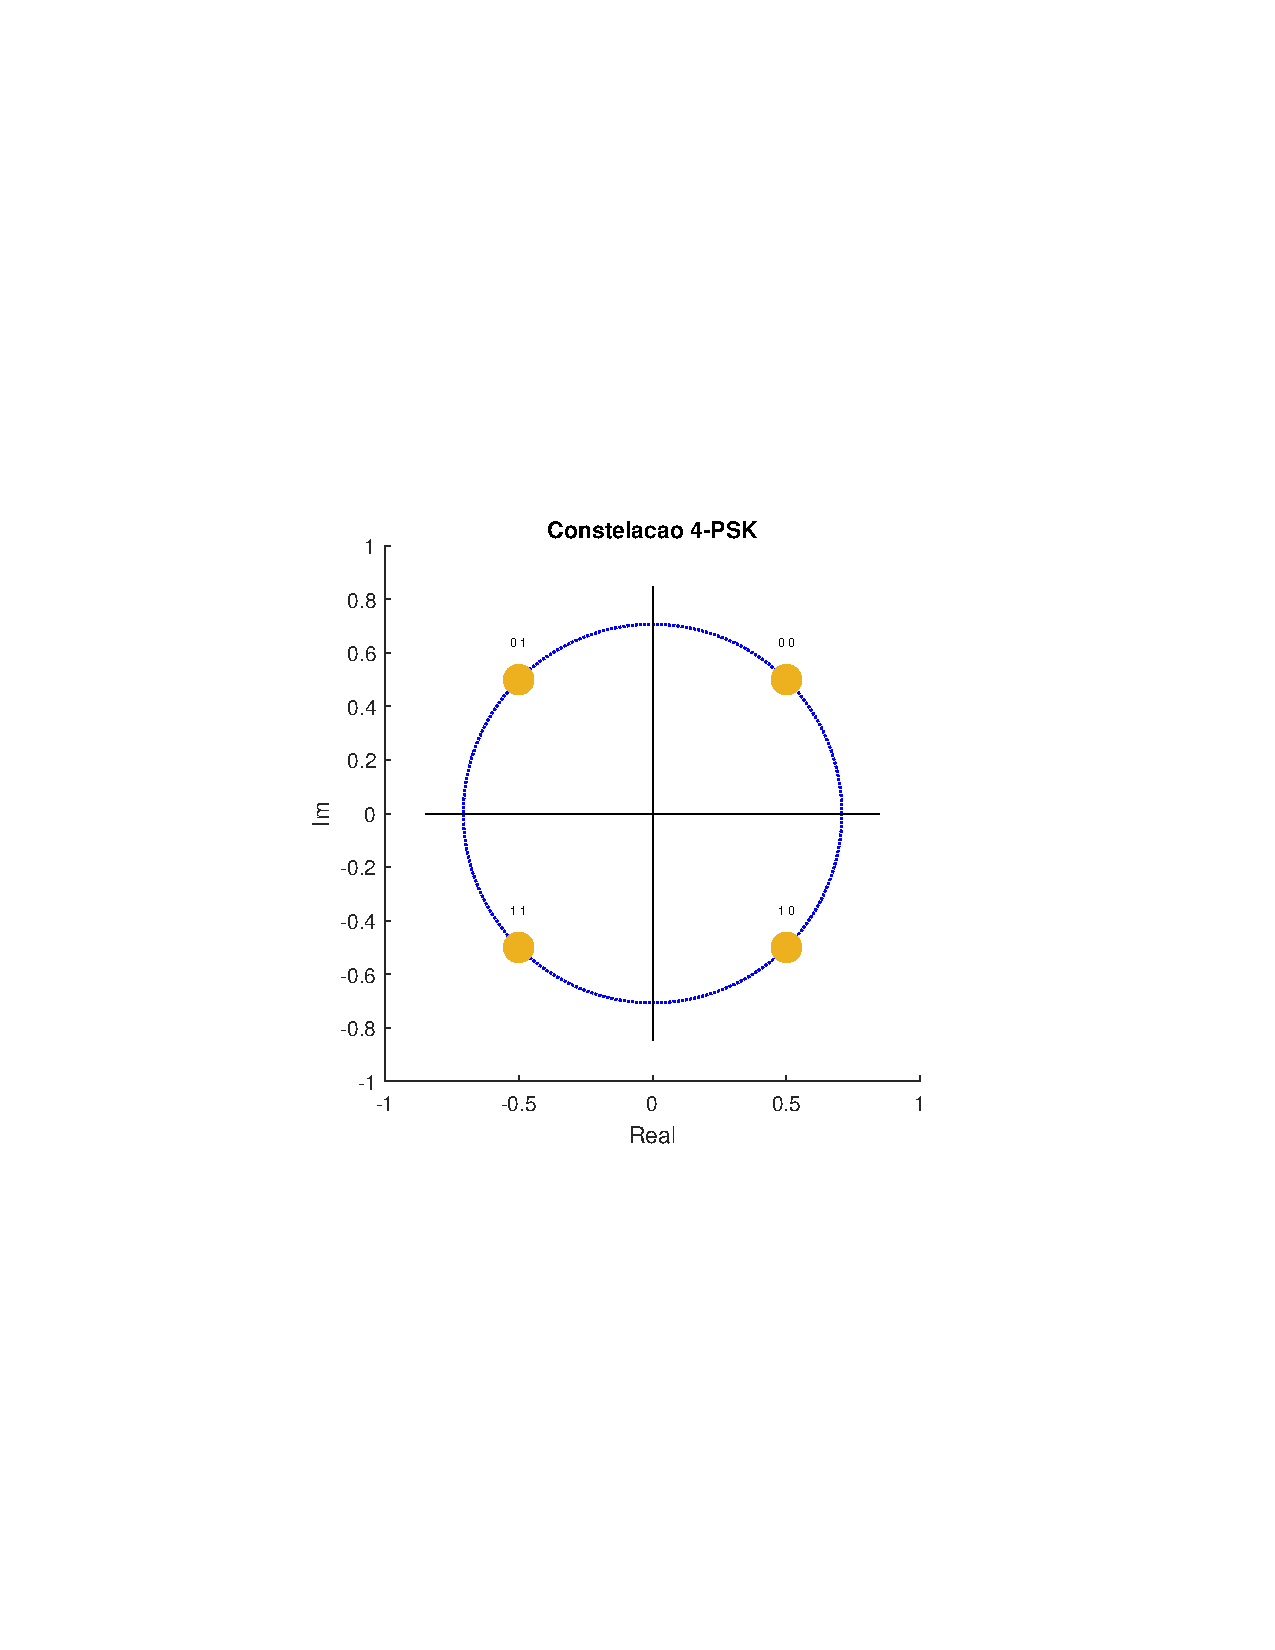
\includegraphics[width=1.0\textwidth,clip=true,trim={1.5cm 8.5cm 1.8cm 8.3cm}]{C:/Users/lukin/Documents/GitHub/Courses-HWs/Sistemas de Comunicacoes Digitais/matlab/problema4/parte1/fig/4_PSK_plot.pdf}
    \caption{Constelação $4$-PSK com codificação de Gray.}
    \label{fig:4_PSK_plot}
\end{figure}

\begin{figure}[!ht]
    \centering
    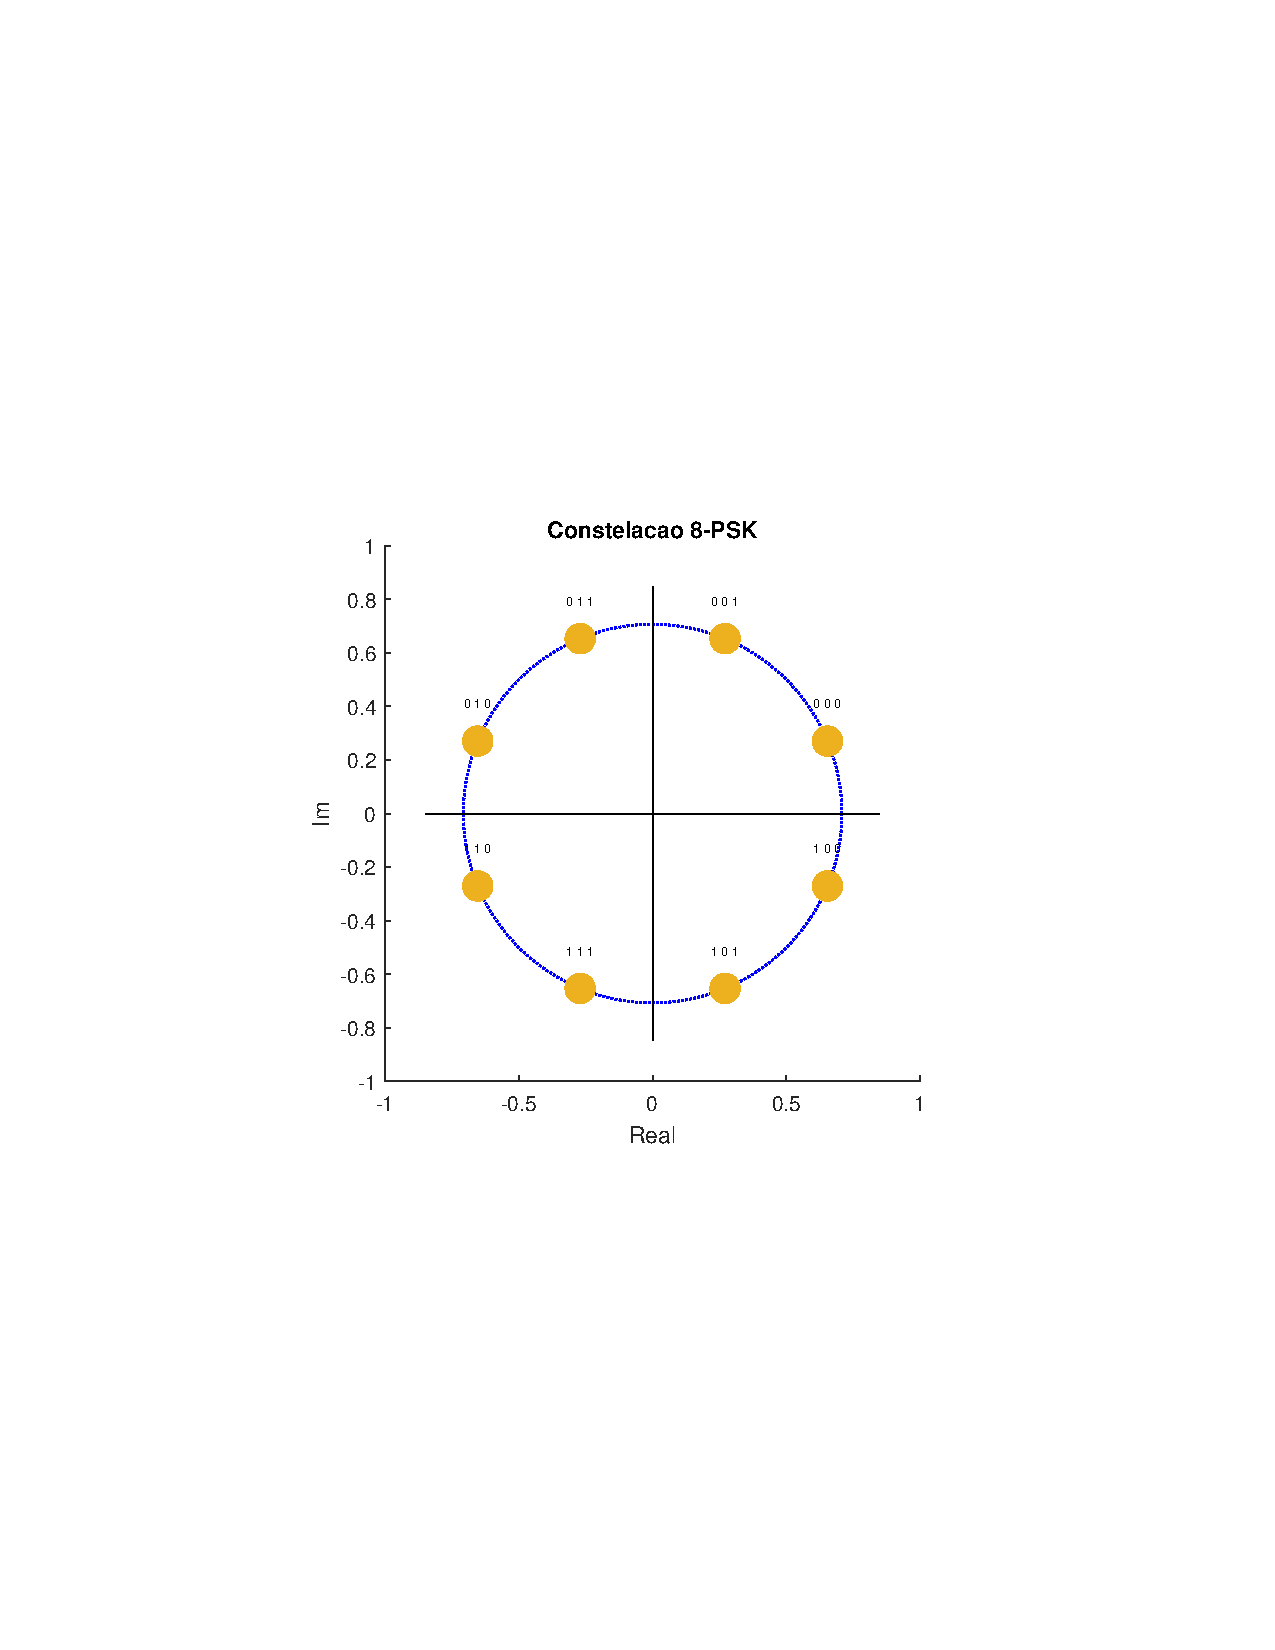
\includegraphics[width=1.0\textwidth,clip=true,trim={1.5cm 8.5cm 1.8cm 8.3cm}]{C:/Users/lukin/Documents/GitHub/Courses-HWs/Sistemas de Comunicacoes Digitais/matlab/problema4/parte1/fig/8_PSK_plot.pdf}
    \caption{Constelação $8$-PSK com codificação de Gray.}
    \label{fig:8_PSK_plot}
\end{figure}



\begin{figure}[!ht]
    \centering
    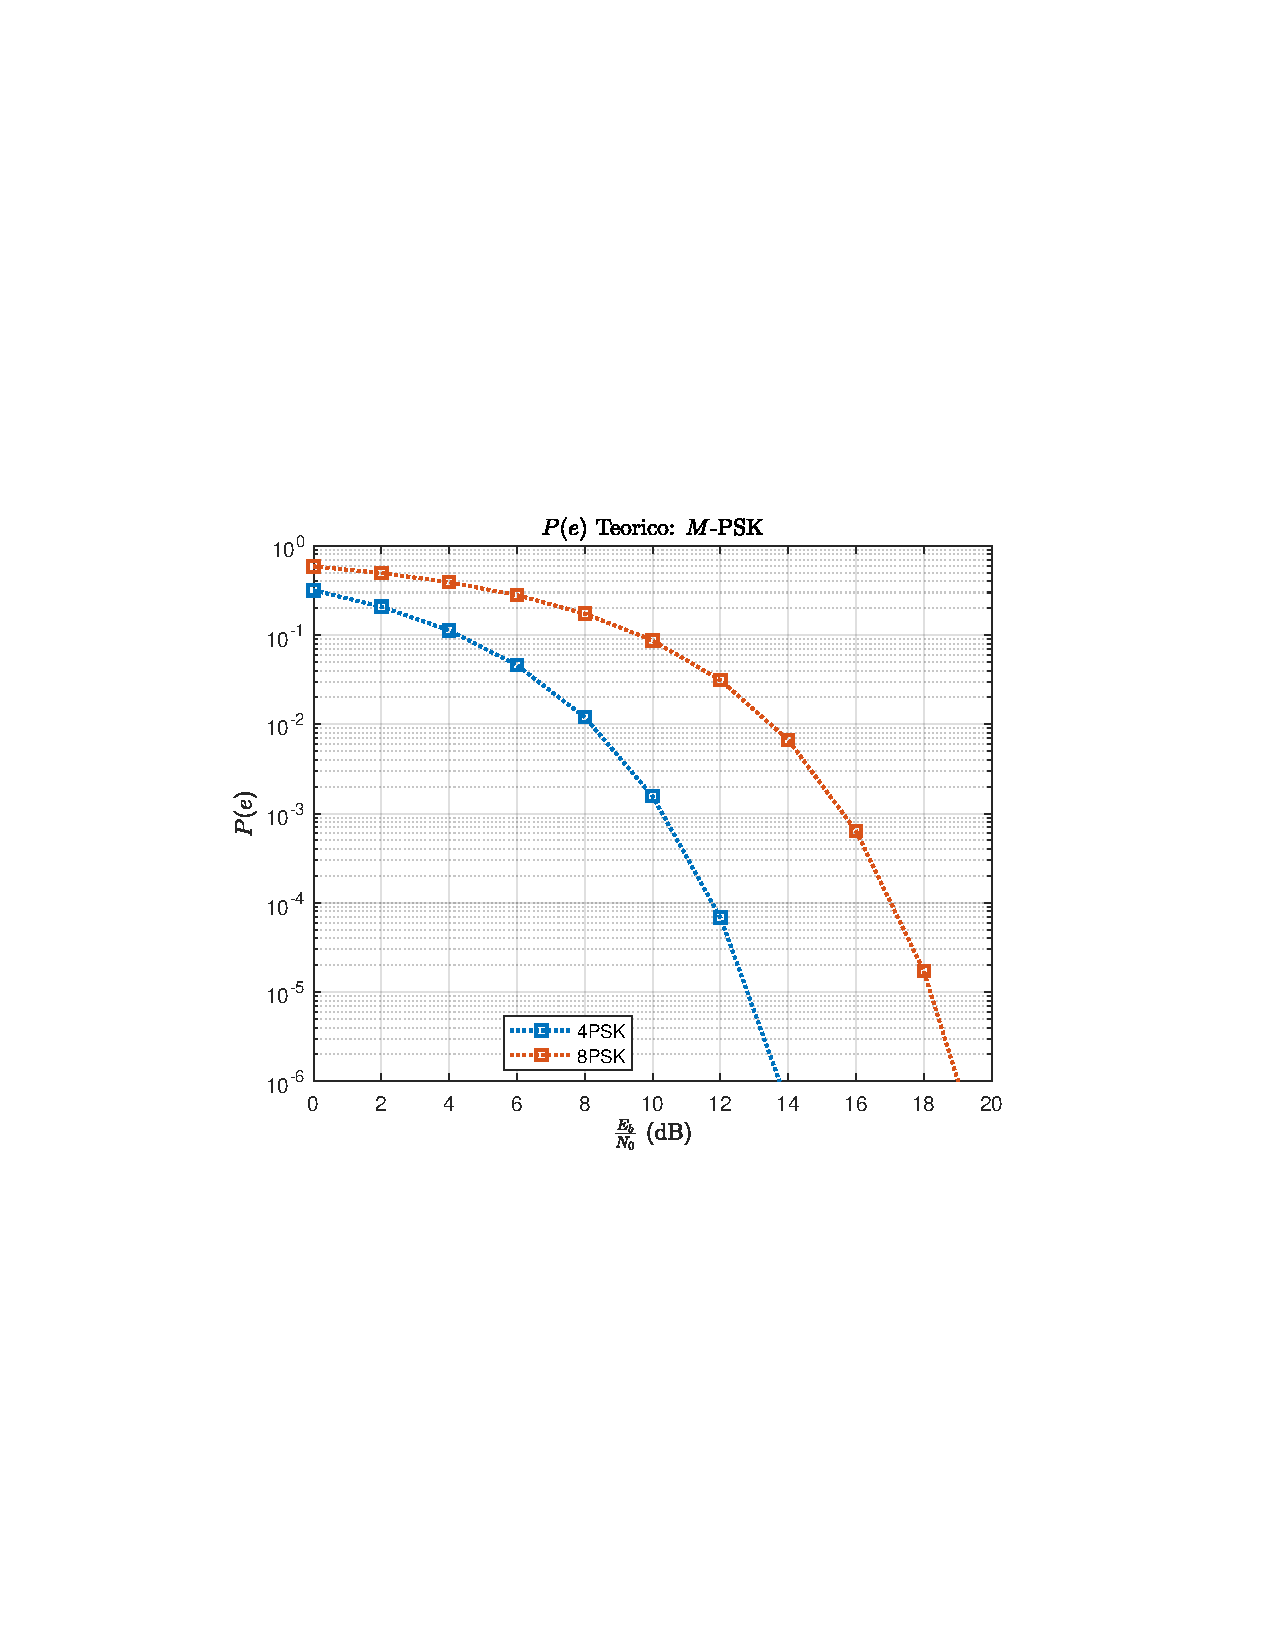
\includegraphics[width=1.0\textwidth,clip=true,trim={1.5cm 8.5cm 1.8cm 8.3cm}]{C:/Users/lukin/Documents/GitHub/Courses-HWs/Sistemas de Comunicacoes Digitais/matlab/problema4/parte2/fig/Erro_Teorico_MPSK.pdf}
    \caption{Probabilidade de erro $(P(e))$ teórico $M$-PSK.}
    \label{fig:Erro_Teorico_MPSK}
\end{figure}


\begin{figure}[!ht]
    \centering
    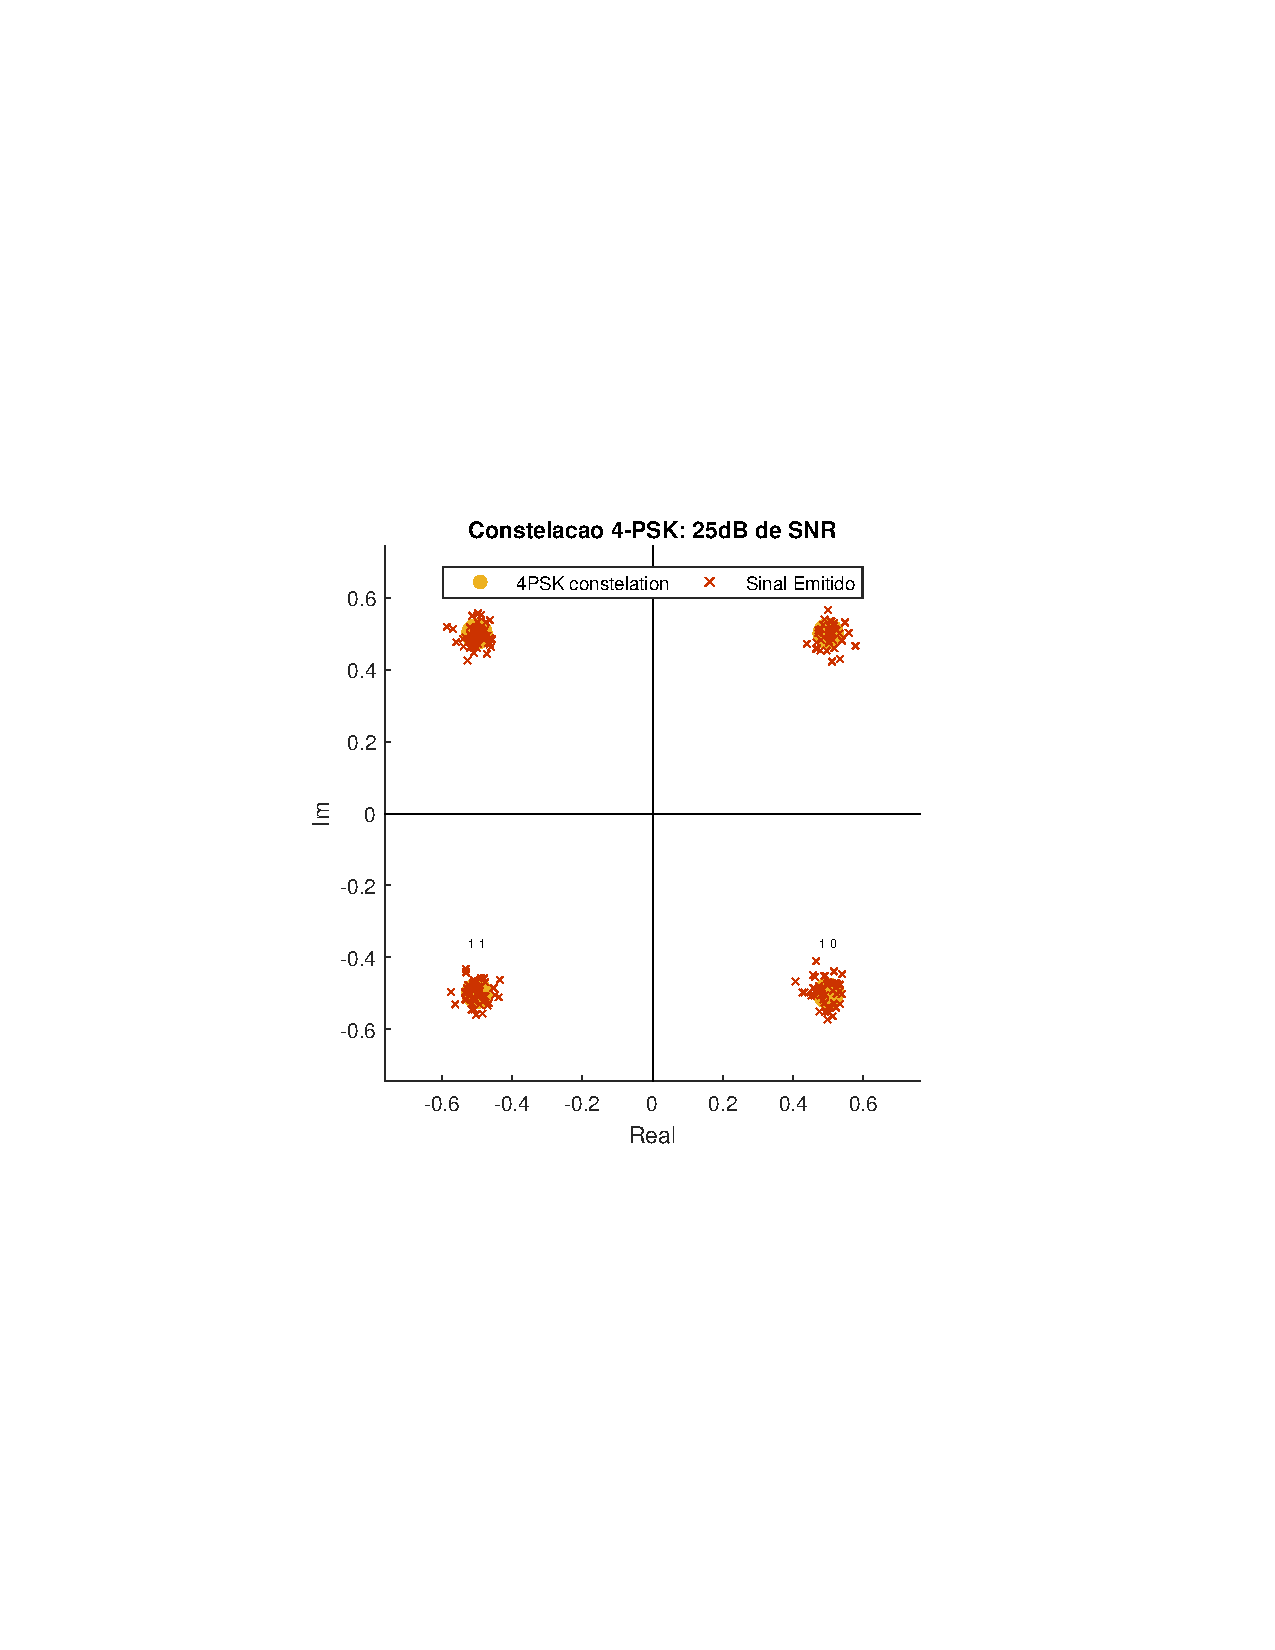
\includegraphics[width=1.0\textwidth,clip=true,trim={1.5cm 8.5cm 1.8cm 8.3cm}]{C:/Users/lukin/Documents/GitHub/Courses-HWs/Sistemas de Comunicacoes Digitais/matlab/problema4/parte3/fig/4PSK_25dB.pdf}
    \caption{Probabilidade de erro $(P(e))$ teórico $M$-PSK.}
    \label{fig:4PSK_25dB}
\end{figure}

\begin{figure}[!ht]
    \centering
    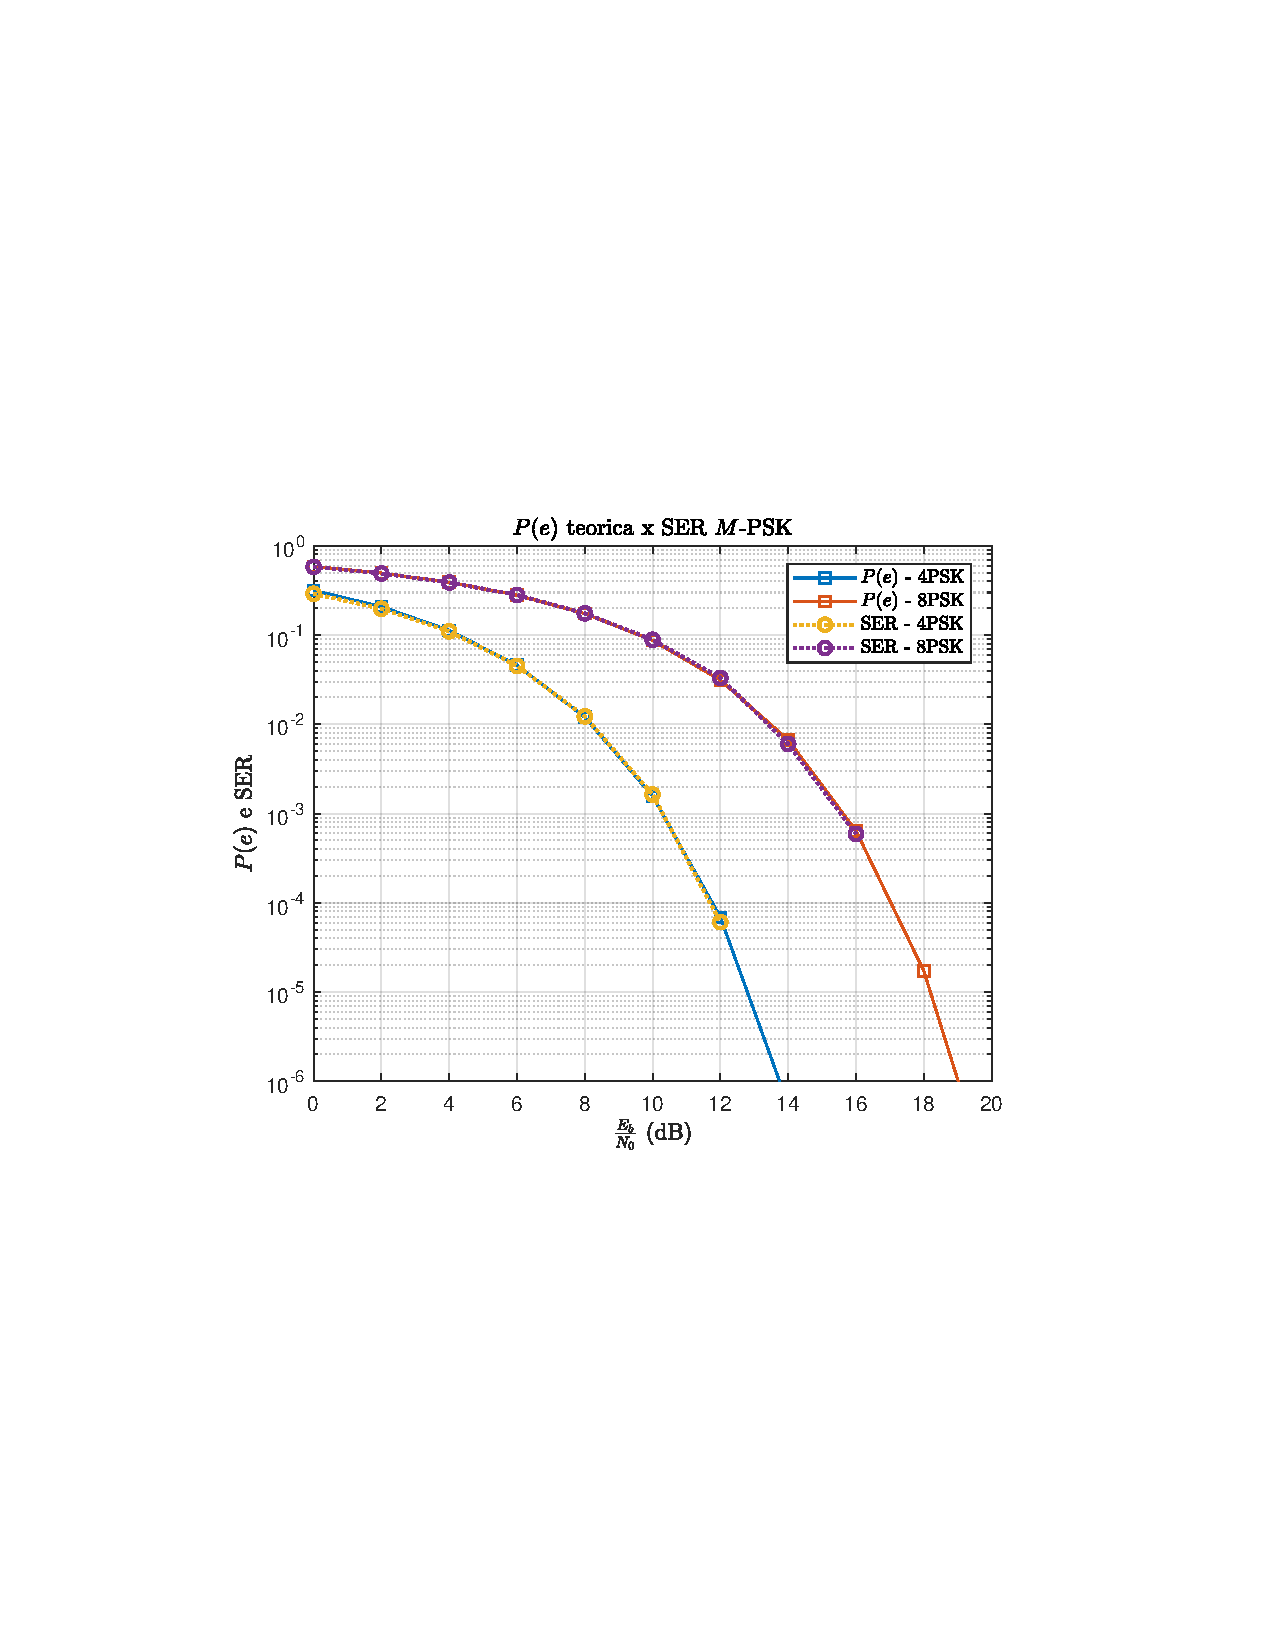
\includegraphics[width=1.0\textwidth,clip=true,trim={1.5cm 8.5cm 1.8cm 8.3cm}]{C:/Users/lukin/Documents/GitHub/Courses-HWs/Sistemas de Comunicacoes Digitais/matlab/problema4/parte3/fig/Erro_teoricaxAWGN_MPSK.pdf}
    \caption{Probabilidade teórica de erro vs. simulação de transmissão $M$-PSK em canal RAGB.}
    \label{fig:Erro_teoricaxAWGN_MPSK}
\end{figure}

